\documentclass[en]{../../../../../../eplexam}

\usepackage{../../../../../../eplunits}
\usepackage[american,RPvoltages]{circuitikz}

\hypertitle{Power electronics}{7}{ELEC}{2660}{2018}{Janvier}{All}
{Louis Devillez}
{Marc Bekemans}

\section{Commenter ce slide /3}

\begin{figure}[H]
  \centering
  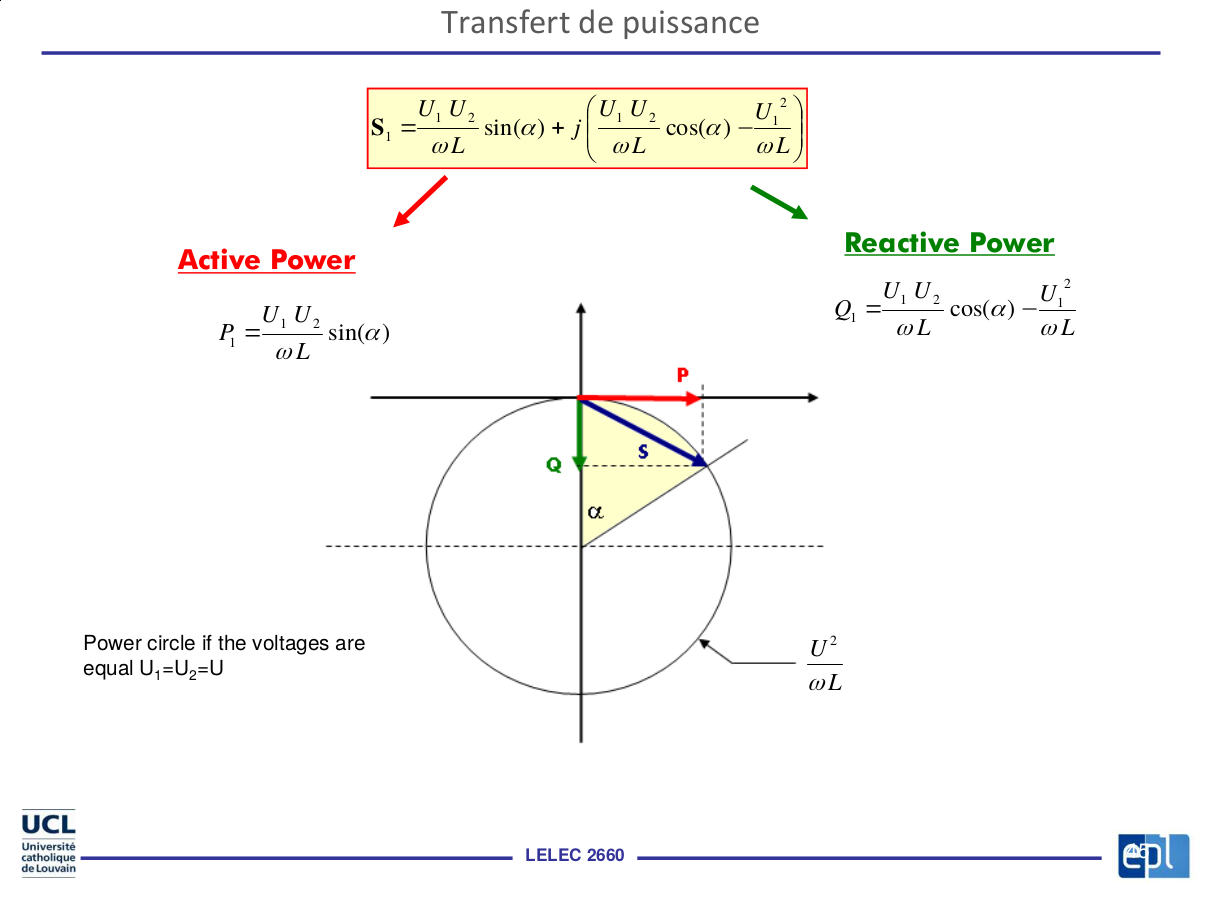
\includegraphics[width=0.65\textwidth]{Q1.png}
\end{figure}

\nosolution

\section{Commenter ce slide /3}

\begin{figure}[H]
\centering
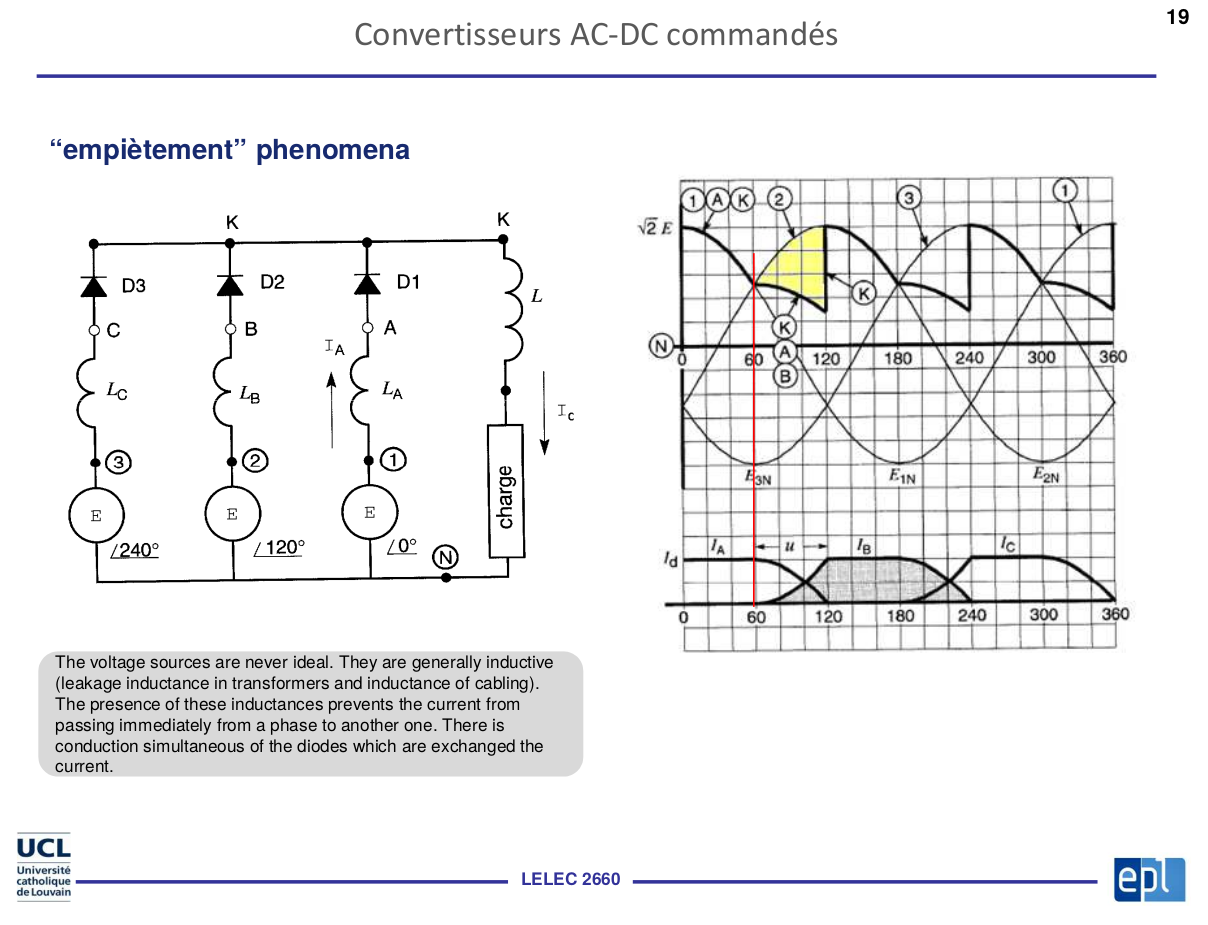
\includegraphics[width=0.65\textwidth]{Q2.png}
\end{figure}

\nosolution


\section{Série des questions à réponses courtes /8}
\begin{itemize}
  \item Un thyristor, à l'état bloqué bloque la tension dans une seule direction. Vrai ou Faux ?
  \item Quel est la relation $V_{out}/V_{in}$ d'un convertisseur forward avec 200 tours au secondaire et 50 tours au primaire ?
  \item Quelle est la tension DC obtenue sans filtrage par un redressement monophasé de la tension présente sur une prise de courant domestique ? Tension de \SI{220}{\volt}.
  \item En régulation de courant ''peak current control``, le convertisseur est stable pour des rapports cycliques inférieurs à 50\% ? Vrai ou Faux ?
  \item La dissipation d'un transistor est de \SI{50}{\watt}. La résistance thermique du boitier (junction-case) est de \SI{0.5}{\kelvin\per\watt}. La résistance de contact avec le radiateur est de \SI{0.1}{\kelvin\per\watt}. La température du radiateur est de \SI{45}{\celsius}. Quelles sont alors les températures de la jonction et du boitier du transistor ?
  \item Quelle est la tension AC (efficace) maximale réalisable par un onduleur monophasé pont complet alimenté en 100V DC ?
  \item Dans un convertisseur forward avec $n_1 = n_2 = n_3$ et $V_{in} = $ \SI{25}{\volt}, quel est la tension maximale bloquée par la diode démagnétisante ?
\end{itemize}

\begin{solution}
  \begin{itemize}
    \item Faux
    \item $$\frac{V_{out}}{V_{in}} = D \frac{n_3}{n_1} = 4D $$
    \item $V_{out} = \frac{220 * \sqrt{2}}{\pi} = \SI{99}{\volt}$
    \item Vrai
    \item $$T_{c} = 45 + 50 * 0.1 = \SI{50}{\celsius}$$
      $$T_j = 45 + 50*(0.1+0.5) = \SI{75}{\celsius}$$
    \item $V {out} = \frac{100}{\sqrt{2}} = \SI{70.7}{\volt}$
    \item $V_{D,max} = V_{in} +  \frac{n_2}{n_1} V_{in} = \SI{50}{\volt}$
  \end{itemize}
\end{solution}

\section{Expliquez, de façon détaillée (figures, diagrammes, équations, explications) le dimensionnement de la capacité de sortie d'un convertisseur DC/DC avec pour objectif de respecter une impédance de sortie définie (variation de tension de sortie pour une variation unitaire de courant de sortie). /7}

\begin{solution}
  Slides 128 à 134
\end{solution}
\section{Convertisseur boost /7}
Avec les caractéristiques suivantes
\begin{itemize}
  \item $V_{in} \in \left[50, 90\right]$
  \item $V_{out}$ regulé à \SI{100}{\volt}
  \item Fréquence de switching: \SI{150}{\kilo\hertz}
  \item Puissance de sortie: \SI{100}{\watt}
  \item Inductance d'entrée: \SI{500}{\micro\henry}
  \item Capacité de sortie: \SI{400}{\micro\farad}
  \item $V_{fdiode} = \SI{850}{\milli\volt}$
  \item $r_{dson,mos} = \SI{150}{\milli\ohm}$
\end{itemize}
\subsection{Établissez la forme de l'onde de courant dans la diode pour la tension d'entrée maximale et minimale}

\begin{solution}
  $$\frac{V_{out}}{V_{in}} = \frac{1}{1-\theta}$$ 
  $$\theta_{min} = 1 - \frac{V_{in}}{V_{out}} = 0.5$$
  $$\theta_{max} = 0.1$$
  $$i_{avg,min} = \frac{i_ch}{1 - \theta} = \SI{2}{\ampere} $$
  $$i_{avg,max} = \SI{1.11}{\ampere} $$
  $$\Delta i_{min} = \frac{V_{in}\theta T}{L} = \SI{0.333}{\ampere}$$
  $$\Delta i_{max} = \SI{0.067}{\ampere}$$
  
  \begin{center}
  	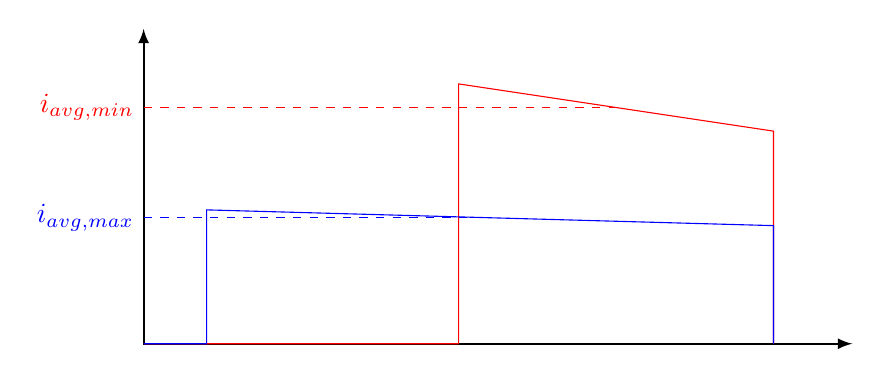
\begin{tikzpicture}
  	\draw [thick, latex-latex] (0,4) -- (0,0) -- (9,0);
  	\draw [red] (0,0) -- (4,0) -- (4,3.3) -- (8,2.7) -- (8,0);
  	\draw [blue] (0,0) -- (0.8,0) -- (0.8,1.7) -- (8,1.5) -- (8,0);
  	
  	\draw [red, dashed] (0,3) node[left]{$i_{avg,min}$} -- (6,3);
  	\draw [blue, dashed] (0,1.6) node[left]{$i_{avg,max}$} -- (4.4,1.6);
  	\end{tikzpicture}
  \end{center}
\end{solution}
\subsection{Établissez la forme de l'onde de courant dans le mosfet pour la tension d'entrée maximale et minimale}

\begin{solution}
	$$\frac{V_{out}}{V_{in}} = \frac{1}{1-\theta}$$ 
	$$\theta_{min} = 1 - \frac{V_{in}}{V_{out}} = 0.5$$
	$$\theta_{max} = 0.1$$
	$$i_{avg,min} = \frac{i_ch}{1 - \theta} = \SI{2}{\ampere} $$
	$$i_{avg,max} = \SI{1.11}{\ampere} $$
	$$\Delta i_{min} = \frac{V_{in}\theta T}{L} = \SI{0.333}{\ampere}$$
	$$\Delta i_{max} = \SI{0.067}{\ampere}$$
	
	\begin{center}
		\begin{tikzpicture}
		\draw [thick, latex-latex] (0,4) -- (0,0) -- (9,0);
		\draw [red] (0,2.7) -- (4,3.3) -- (4,0) -- (8,0);
		\draw [blue] (0,1.5) -- (0.8,1.7) -- (0.8,0) -- (8,0);
		
		\draw [red, dashed] (0,3) node[left]{$i_{avg,min}$} -- (2,3);
		\draw [blue, dashed] (0,1.6) node[left]{$i_{avg,max}$} -- (0.4,1.6);
		\end{tikzpicture}
	\end{center}
\end{solution}

\subsection{Établissez le pire cas de dissipation (perte en conduction seulement) dans la diode et le transistor}

\begin{solution}
	Les dissipations dans la diode ont la forme
	$$P = V_jI_f + R_f I_f^2$$
	$$P = V_j I_{avg} + R_f I_{RMS}^2$$
	La valeur RMS pour $V_{in} = 90$ est plus faible et donc il y a moins de pertes.
	
	Les dissipations le transistor ont la forme 
	$$P = R_{ds} I_{rms}^2$$
	La valeur RMS pour $V_{in} = 90$ est plus faible et donc préférable
\end{solution}
\section{Déterminer le circuit dual d'un convertisseur buck-boost /3}

\begin{solution}
  \begin{center}
    \begin{circuitikz}
      \draw (0,0) node[nmos](nmos){};
      \draw [fill=white] (-0.65,0) circle(0.05);
      \draw (nmos.S) to [D] ++ (0,-1.5) -- ++ (1.5,0) to [I] ++ (0,3.5)  -| (nmos.D);
      \draw (nmos.D) ++ (1.5,0.458) to[C] ++(2,0) to [D] ++ (0,-3.5) -- ++(-2,0); 
      \draw (nmos.D) ++ (3.5,0.458) to[L] ++ (2,0) to [R] ++ (0,-3.5) -- ++ (-2,0);
    \end{circuitikz}
  \end{center}
\end{solution}
\section{}
Établissez les équations d'états d'un convertisseur boost avec le rapport cyclique $\theta$ comme paramètre /4

\begin{solution}
  \begin{center}
    \begin{circuitikz}
      \draw (1,0) to[nos,mirror] (3.5,0) to [C,v=$V_1$,l=C] ++ (0,-2) -- ++ (-1.25,0)-- ++ (0,1.6);
      \draw (3,0) -- ++ (2,0) to [R] ++ (0,-2) -- ++ (-2,0);
      \draw (1,0) to [L, mirror, i<=$i_1$,l=L] ++ (-2,0) to[V] ++(0,-2) -- ++ (3.3,0);
    \end{circuitikz}

    \bigbreak
    \begin{tabular}{c|c|c}
    &ON&OFF\\
    \hline
      $C\cfrac{dV_1}{dt}=I_c$&$-I_{ch}$&$I_1 - I_{ch}$\\
      $L\cfrac{dI_1}{dt}=V_l$&$E$&$E-V_1$
    \end{tabular}
  \end{center}


  $$\begin{bmatrix}
    \cfrac{dV_1}{dt}\\
    \cfrac{dI_1}{dt}
    \end{bmatrix} = \begin{bmatrix}
      0 & \cfrac{1-\theta}{C}\\
      0 & \cfrac{-(1-\theta)}{L}
    \end{bmatrix} \begin{bmatrix}
      V_1\\
      I_1
  \end{bmatrix}$$
\end{solution}

\section{Question bonus: dimensionner l'inductance de magnétisation (vu depuis le secondaire) and la capacité de sortie d'un convertisseur flyback dans le but de limiter le ripple de sortie à \SI{100}{\milli\volt} /+5}
\begin{itemize}
  \item $V_{in} = \SI{50}{\volt}$
  \item $V_{out} = \SI{200}{\volt}$
  \item$ F_{sh} = \SI{100}{\kilo\hertz}$
\end{itemize}   

Rmq: Je ne suis pas certain que l'énoncé soit complet.

\nosolution

\end{document}
